\section{Experimental Results}
\label{sec:eval} 
In this section, we first give some statistics of
our corpus and the extracted causality network, and evaluate the
quantity and quality of the cue patterns used in the extraction. 
%\ZY{Futhermore, we primarily evaluates the causality 
%strength metric proposed in this paper and the quality 
%of our causality network haversting from large web corpus.}
We then compared our results on the main COPA task against a number of
existing works using various other data sources and knowledge bases.
Next, we evaluate causality reasoning
on two additional tasks using the data from ConceptNet 4 to
further showcase the power of our framework.
%To show the coverage of our causality network, 
%we use causality knowledge of ConceptNet in a reasonable way 
%and compares with its results on COPA task.
Finally, we demonstrate our network's ability to identify causal directions
using annotated corpus of SemEval-2010 task 8, despite being
agnostic about the context of the input word pairs.
We release the evaluation data used in these experiments 
at \url{http://202.120.38.146/causal}.

\subsection{Data Set and Extraction of Causality Network}
\label{sec:causalnet}
\begin{figure}[th]
\centering
\epsfig{file=pattern1.eps, width=1.05\columnwidth}
%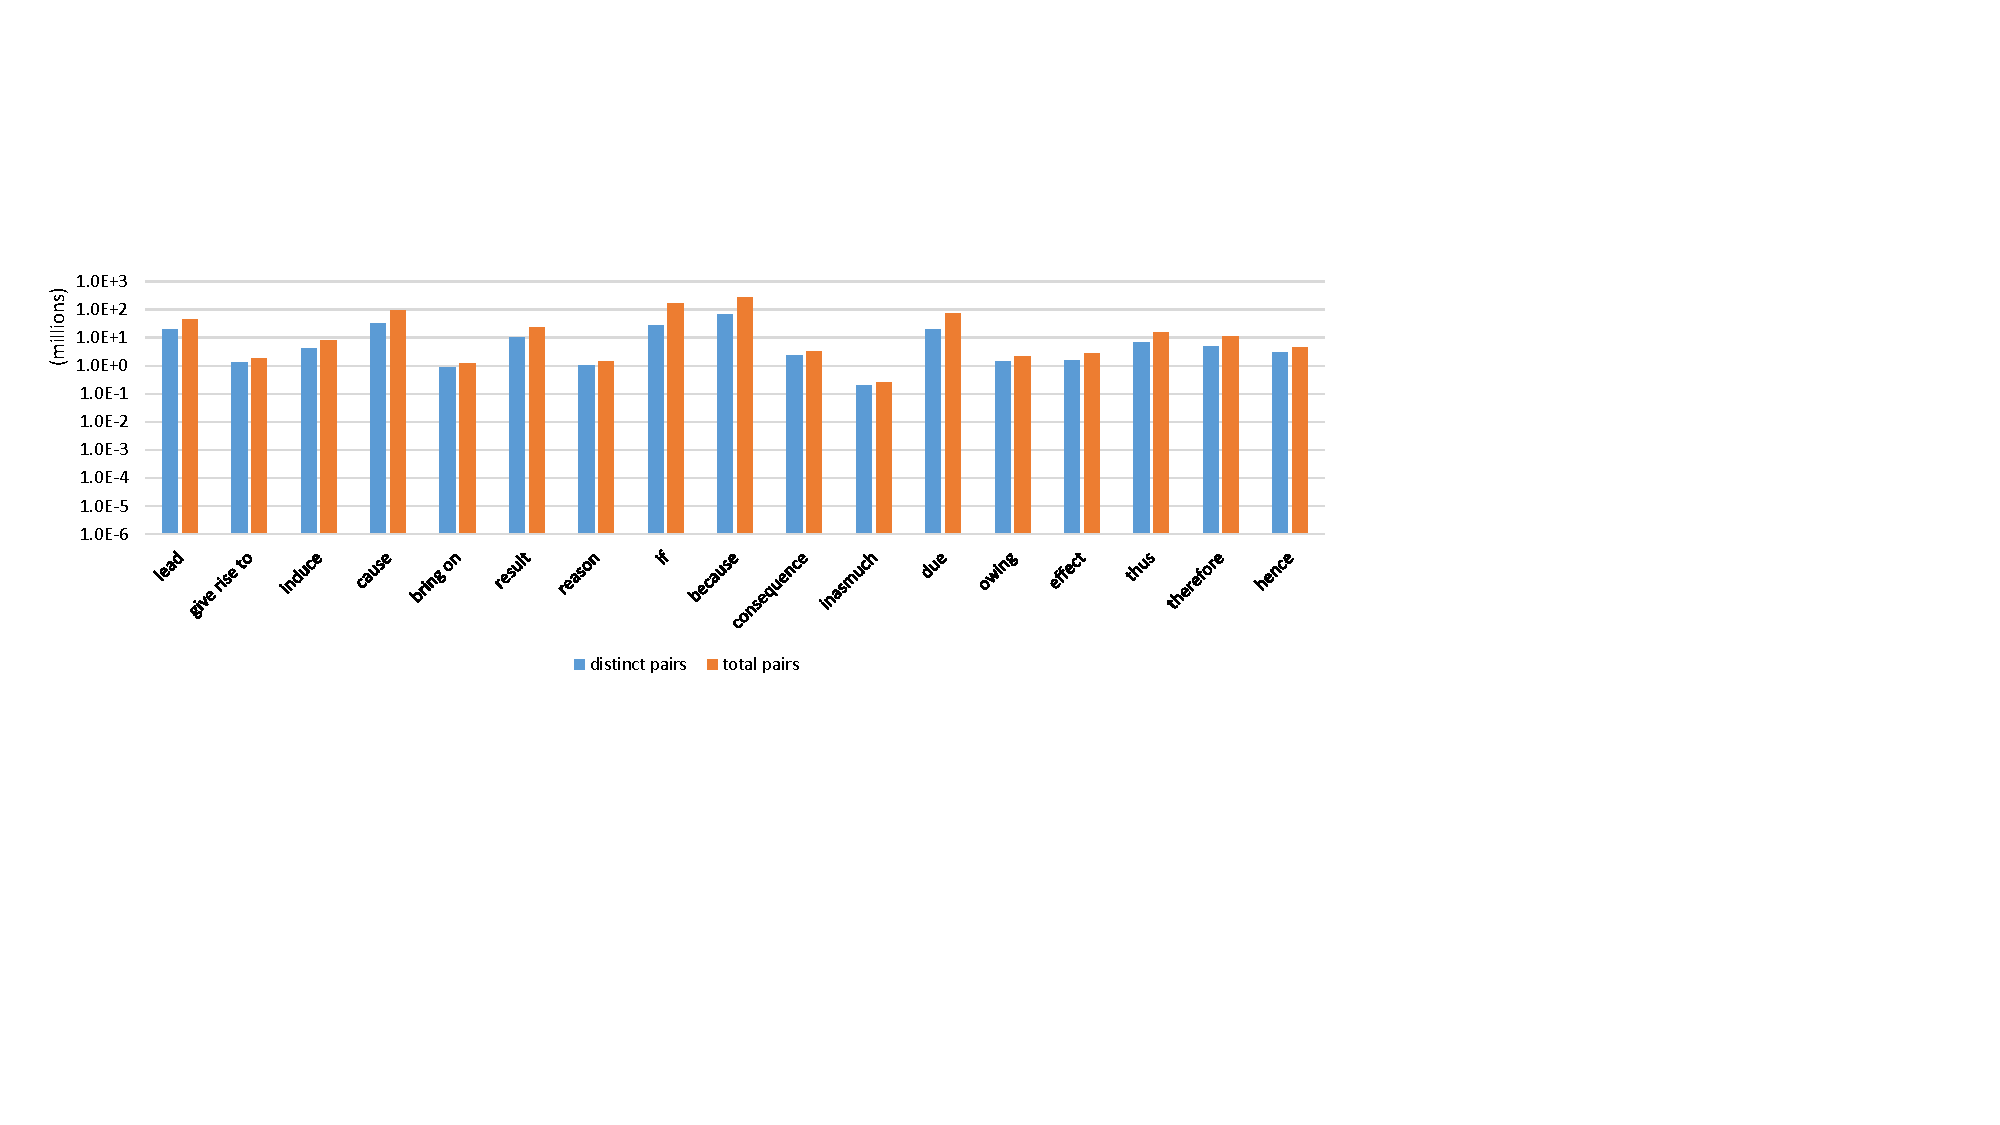
\includegraphics[width=2\columnwidth]{pattern.pdf}
\caption{Number of (distinct) pairs extracted by cues}
\label{fig:pattern1}
\end{figure}
We extracted our term causality network, which we call ``CausalNet''
for convenience in this section, from a large web text corpus (approximately
10TB), %The snapshot was generated in February, 2013
which contains about 1.6 billion web pages.
We extract 62,675,002 distinct causality evidences (e.g., causal pairs
or edges in CausalNet) from this corpus. 
The average frequency of these evidences is 10.54.
The number of unique lemmatized terms (nodes)
in these evidences is 64,436, covering 41.49\% (64,436/155,287) of the
words in WordNet. 

As a comparison, we separately extracted an 
``event-based'' CausalNet using dependency relations 
such as \emph{advmod} and \emph{dobj}. 
Only bigram-phrases that match these relations and appear more than
20,000 times in the corpus are considered events; otherwise they are split
into words and paired up as before. 
The average frequency on the edges of this event-based CausalNet
is 1.59, much smaller than the orginal CausalNet. Therefore, subquent 
experiments are done on the term-based CausalNet.

The 53 causal cues we used can be grouped into 17 sets, each
containing cues of the same meaning or lemma form but with different
tenses. Word pair distribution over these sets is shown in Figure
\ref{fig:pattern1}. The blue bars (left) are the number of distinct
pairs and the orange ones (right) show the total number of pairs.
Inter-sentence cues like ``if'' and ``because'' harvested the
largest number of pairs. But more specific patterns such as
``reason'' and ``inasmuch'' find more diverse pairs, since the
number of distinct pairs is relatively large compared to the total
pairs extracted.

\begin{figure}[th]
\centering
\epsfig{file=pattern3.eps, width=1.05\columnwidth}
%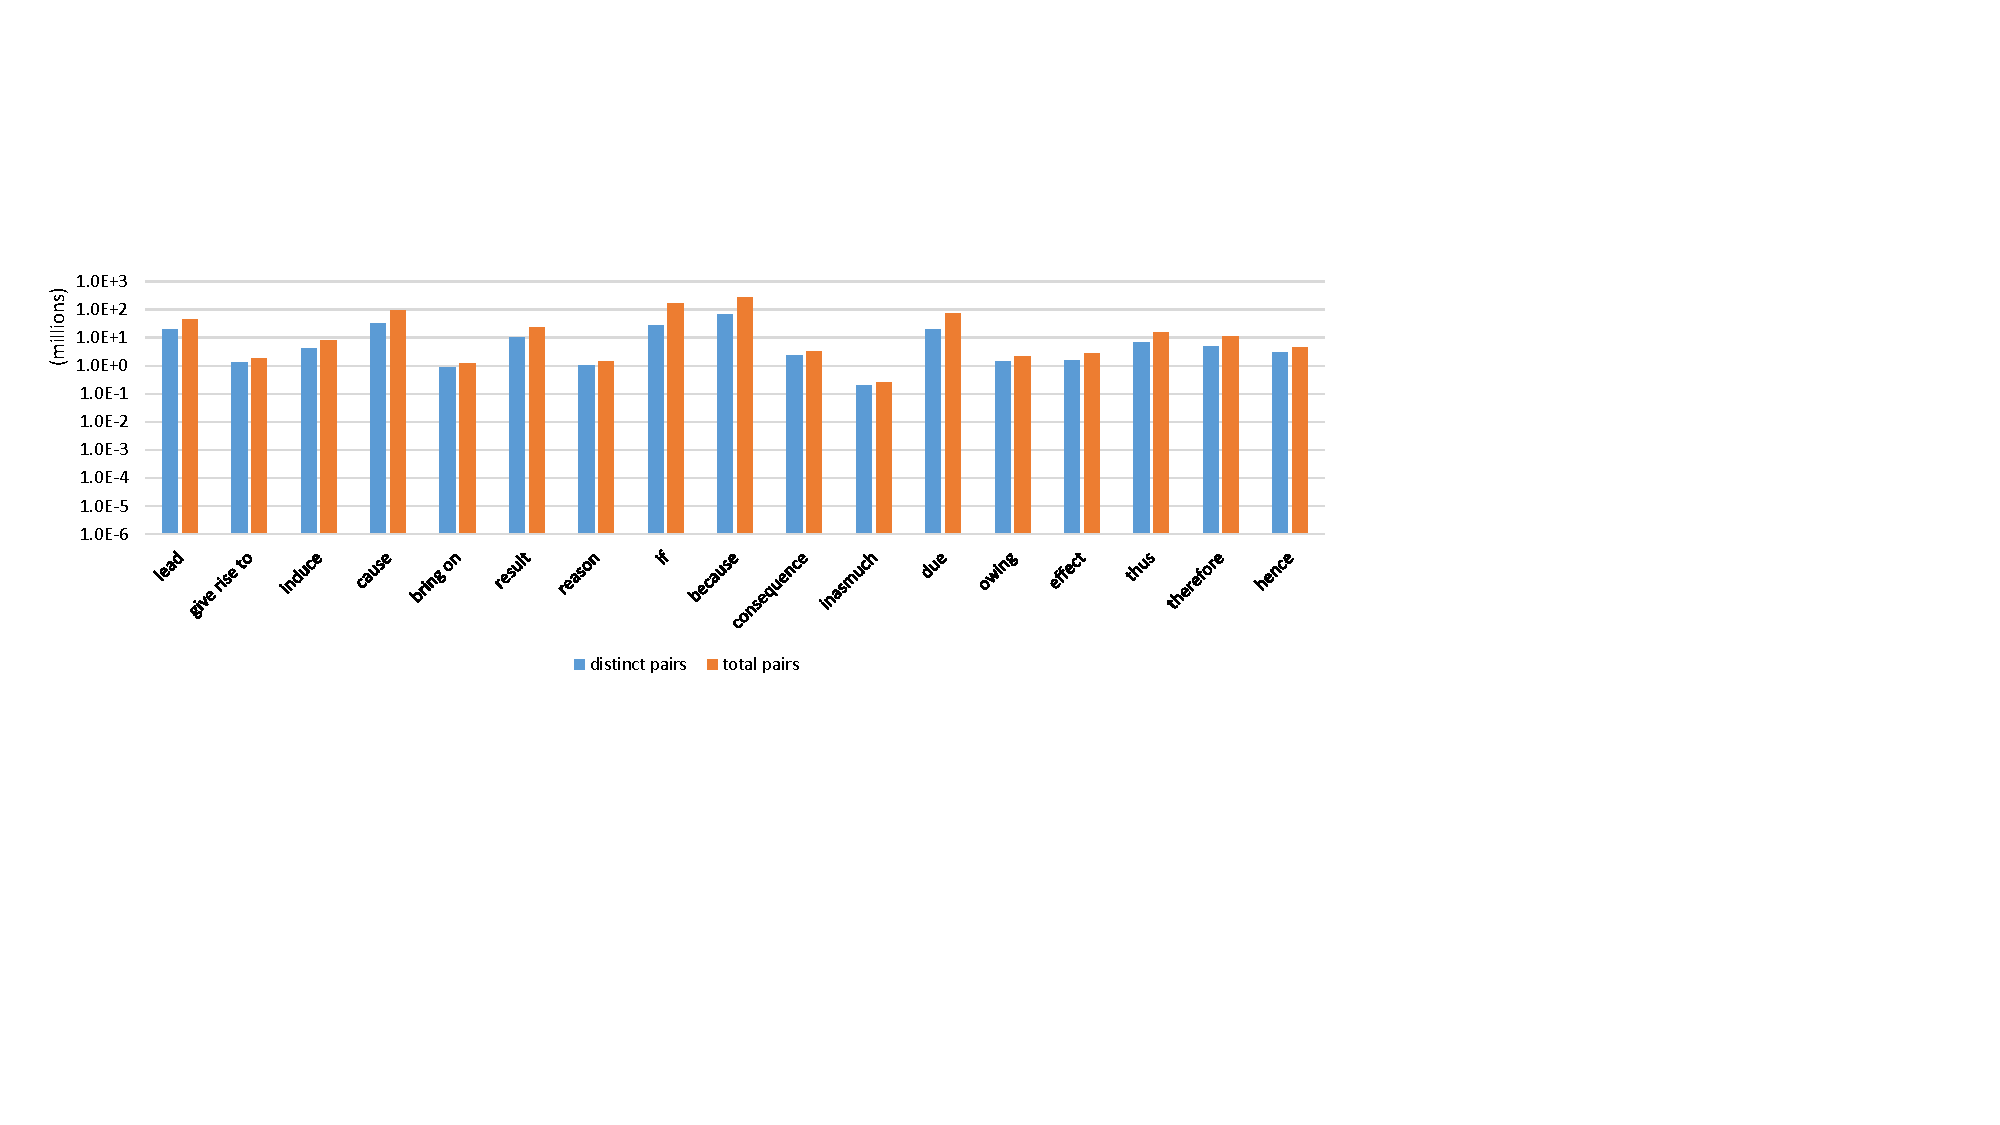
\includegraphics[width=2\columnwidth]{pattern.pdf}
\caption{Number of causal vs. non-causal pairs from ConceptNet covered by cues}
\label{fig:pattern2}
\end{figure}

To evaluate the quality of the causal cues, we make use of the
manually labeled causal events in
ConceptNet~\cite{liu2004commonsense} as ground truth. ConceptNet 4
contains 74,336 unlemmatized English words, forming
375,135 unique concepts, which are connected by 610,397 relation edges.
Only some of these relations encode causal knowledge,
such as ``Causes'', ``CausesDesire'' and ``HasPrerequisite''.
The total number of such causal relation is 52778.
%This is significantly smaller than our
%CausalNet in scale, especially in terms of number of edges.
%%Otherwise, relations are more sparse in ConceptNet.
%We randomly collect 100 causal even pairs and 100 non-causal event pairs from
%ConceptNet,
%based on feedbacks from human volunteers of OMCS project, who cast positive
%votes for each \emph{Causes} relationship that is causal, and
%negative for that is not. 
Since the pairs from ConceptNet contain
phrases and not just words, we consider a pair ($x$, $y$) to be covered by a
causal cue, if at least one word $u$ from $x$ and another word $v$ from
$y$ are extracted as cause word and effect word by the cue
from the web corpus.
\figref{fig:pattern2} shows that in general, our cues can
effectively distinguish between positive and negative causal pairs,
with the exception of ``hence'' and ``consequence'', both of which
represent relatively coarse-grained entailment relation.
Particularly good cues to distinguish the positive and negative
pairs are ``due to'' and ``induce''.

\subsection{End-to-end Evaluation on COPA}
COPA task consists of 1000 causal reasoning questions, divided into
development question set and test question set of 500 each.
%The authoring methodology of COPA ensured sufficient breadth of the topics
%in the question set. Each question in COPA data set was validated
%by two raters with high inter-rater agreement.
The incorrect alternative was purposely set semantically
close to the premise, which makes this task more difficult for
purely associative methods. In this experiment, our parameter $\lambda$
was trained on the development set.
All the reported results are on test set.

To show the usefulness of our causality metric, denoted as $CS$, 
we compare the end-to-end results on COPA with the 
best known PMI statistics on the web corpus. Here we use the 
implicit cause patterns adopted previous work, that is, if a pair of
terms ($i$, $j$) is extracted from text. $i$ is considered the cause
if it appears before $j$ in the text, and vice versa.
To solve COPA question with PMI, we pair the terms from
premise and alternative and choose the alternative 
with a higher PMI.
\tabref{tab:evaluation} shows that at
%the best $CS$ (i.e., $CS_{\lambda=0.5}$) results
$\lambda = 0.5$, the best $CS$ results
(64.8\%) outperforms PMI with any window sizes.

\tabref{tab:evaluation} also compares $CS_{\lambda=1.0}$ on CausalNet 
with several other approaches. 
PMI Gutenberg~\cite{roemmele2011choice} uses PMI statistic calculated 
from Project Gutenberg (16GB of English-language text). 
%They pair the words from
%premise and alternative and choose the alternative with a higher
%PMI. Their result is the best with a window size of 5. 
UTDHLT~\cite{goodwin2012utdhlt} is the
result of SemEval-2012 Task 7 systems. They proposes two
approaches. The first one uses PMI over bigrams from LDC Gigaword corpus
(8.4 million documents) as a
feature. The second one treats the task as a classification
problem and combine the features used in the first approach with
some additional features to train an SVM model. 
%The author only provides the score of test set such that results for
% development and all set could not be reported.
The ConceptNet approach was our own baseline to illustrate the power of
human curated knowledge. Here we fuzzy match
the events or concepts from ConceptNet in COPA sentences, and then compute
the causal strength between two COPA sentences by the scores associate with
causal relations in ConceptNet. 
23 out of 500 questions 
on COPA test split are matched by ConceptNet, 
and 18 of them are correctly answered, 
by computing the causality strength between two COPA sentences 
from the scores associate with causal relations in ConceptNet.
We just randomly select an answer 
for mismatched questions.
The last PMI method~\cite{gordon2011commonsense}, which was also the 
state-of-the-art previoulsy (65.4\%), uses a large corpus of
personal stories (37GB of text) with a window of 25.
All competing systems were assessed based
on their accuracy on the 500 questions in the COPA test
split~\cite{gordon2012copa}. Results show that our new metric 
$CS_{\lambda=1.0}$, 
when used together with the automatically harvested CausalNet 
achieve significantly better accuracy on the COPA task.
%The differences in accuracy between ours and Gordon's PMI \ZY{on web corpus} are
%statistically significant at $p<0.01$, calculated using 
%stratified shuffling \cite{resampling1989computer}. 

%That is if term $i$ appears before term $j$ in text,
%we take $i$ as the cause role and $j$ as the effect role, 
%extracting $(i_c,j_e)$ as the causlity evidence.
%Futhermore, we apply the new metric of causality strength (i.e., $CS$),
%using our causality network on COPA evaluation, achieving 70.2\% 
%highly outperforms best known results. 

\begin{table}[th]
\small
\centering
\caption{COPA results comparison}
\label{tab:evaluation}
\begin{tabular}{llccc}
\hline
Data Source & Methods & Accuracy(\%) \\
\hline
Web corpus & PMI (W=5) & 61.6\% \\
& PMI (W=10) & 61.0\% \\
& PMI (W=15) & 60.4\% \\
& PMI (W=25) & 61.2\% \\
& {\bf $CS_{\lambda=0.5}$} & {\bf 64.8\%} \\
\hline
Gutenberg & PMI (W=5)  & 58.8\% \\
& PMI (W=25) & 58.6\% \\
\hline
LDC Gigaword & UTDHLT Bigram PMI & 61.8\% \\
 & UTDHLT SVM & 63.4\% \\
\hline
ConceptNet & Fuzzy match & 51.3\% \\
\hline
1-Million Stories & PMI (W=25) & 65.2\% \\
10-Million Stories & PMI (W=25) & {\bf 65.4\%} \\ \hline
%\ZY{PMI 10TB web corpus (W=xx)} & \ZY{xxx}\% \\
%CausalNet w/o events & 67.6\%  \\
CausaNet & {\bf $CS_{\lambda = 1.0}$ } & {\bf 70.2} \%  \\
\hline
\end{tabular}
\end{table}



%\ZY{Note that, \textit{Causality Network} is extracted from 10T web corpus 
%by causal indicators. Using Causality Network as data source means we 
%leverage explicit causality encoded in the web corpus. 
%Thus, in \tabref{tab:evaluation}, using data source of 10T web corpus means 
%leverage the implicit causlity encoded in the web corpus.
%}
\cut{%%%%%%%%%%%%%%%%%%%%%%
The parameter $\lambda$ of our causality metric 
weights the necessity and sufficiency causality evidences of 
the data source.
Therefore, to apply our causality metric using different data source, 
we retuned the parameter $\lambda$ on the dev set, 
from 0.0 to 1.0 with a step of 0.1.
From \tabref{tab:evaluation}, we observe the following: 
1) $CS$ performs better than 
PMI on the same causality data source (10T web corpus), which 
suggests that our metric is useful in 
computing causality strength.
2) The best tuned $\lambda$ of \textit{Causality Network},
the explict causality evidences extracted from 10T web corpus) is 1.0,
and that of \textit{discourse causality}, the implicit cauaslity 
evidences encoded in 10T web corpus, is 0.5.
\textit{causality network} is the explicit causality evidences 
generating from 10T web corpus, which identified with preciser 
cause/effect roles. 
That means these two different causality data source 
carries different propotional neccessity and sufficiency causality 
evidences. The explicit causality evidences extracted by 
causal indicators (e.g., cause, because) are almost 
necessity causality as we discussed in \secref{sec:reasoning}.
Thus, the best $\lambda$ using \textit{Causality Network} is close to 1.0.
And the implicit causality in discourse encode both necessity and sufficiency 
causality, and therefore its best $\lambda$ on dev set is smaller, which is
0.5. Note that, best choice of $\lambda$ for 10T web corpus is 0.5 does not 
means the propotion of necessity causality evidences in that 
data source is 50\%. 
We assume that $\gamma$ is the true weight
that weighting for the importance 
of necessity and sufficiency causality in causality modeling.
If we can model necessity and sufficiency causality 
correctly, then $\lambda$ is exactly the value of $\gamma$.
That means if we use $f_{nec}(i_c,j_e)$, 
the frequency of $(i_c,j_e)$ encodes necessity causality, to replace $f(i_c,j_e)$ 
in \eqnref{eq:csnec}, we can correctly model the neccessity causality 
encodes in $(i_cj_e)$, similar to sufficiency causality in \eqnref{eq:cssuf}. 
However, we can not recognize the evidences encodes the necessity causlity or 
sufficiency causality. We combine $\gamma$ together with the evidences bias of 
data source as weighting parameter $\lambda$.
Thus, $\lambda$ reflects both the importance of necessity/sufficiency evidences 
and the quantity bias of these two kinds of evidences extracted from data source.
3) PMI on personal stories outperforms both PMI and CS applied on 10T web corpus, 
which suggests that personal stories is a better implicit causality source than 10T web corpus.
However, CS on Causality Network outperforms all the existing approaches. 
It shows that CS is more powerful when given preciser cause/effect roles. 
That means CS applied on explicit causality knowledge is more proper. 
Although, CS applied on implicit causlity source (10T web corpus) achieves competitive results.
We argue that CS is a useful metric for causality reasoning.
}%%%%%%%%%%%%%%%%%%end of cut %%%%%%%%%%%

%Also, we tuned $\lambda$ on the development set, weighting strengh of 
%necessity and sufficency causality by capturing 
%the implicit causality evidences encoded in discourse of web corpus.
%It shows that setting $\lambda$ to be 0.5 is the best choice.
%Proper value of $\lambda$ for explicit evidences carried by 
%our causality network is close to 1.0 as we will see later 
%in Table (?). That is because the explict evidences extracted by 
%causal indicators (e.g., cause, because) bias towards necessity causality 
%as we discussed in sec (?). }


%We tuned the parameters $\alpha$ and $\beta$ on the development set by
%attempting all combinations of values from 0 to 1.0 with a step of
%0.1. The best combination was empirically found  to be $\alpha=0.4$,
%$\beta=0.3$. Note that, setting parameter $\alpha=0$,
%$\beta=0$ models the causal strength to be exactly the product of
%two conditional probabilities. Another extreme would be setting
%$\alpha=1$, $\beta=1$, where the causal strength becomes \eqnref{eq:pmi2},
%which is actually the square of PMI with causal directions
%itself without logarithm.

%Our method without event enhancement
%serves as a baseline; it does not detect any events or
%boost the strength of any word in the
%input sentence but merely uses the causal network and the
%causal strength scores between words.

%We compare our system (with and without event enhancement step)
%with a number of state-of-the-art systems, and report the results in
%\tabref{tab:evaluation}.
%All competing systems were assessed based
%on their accuracy on the 500 questions in the COPA test
%split~\cite{gordon2012copa}.

%but we also show the accuracy on development set and all questions.
%The overall score is the mean value of development and test set because the two
% sets have equal number of examples.
%Table~\ref{tab:evaluation}
%\begin{table}[th]
%\small
%\centering
%\caption{COPA results comparison}
%\begin{tabular}{|l|c|c|c|}
%\hline Methods & Dev & Test & All  \\ \hline \hline
%PMI Gutenberg (W=5)\cite{roemmele2011choice} & 57.8\% & 58.8\% & 58.3\% \\
%UTDHLT Bigram PMI\cite{goodwin2012utdhlt} & - &61.8\% & - \\
%UTDHLT SVM Combined\cite{goodwin2012utdhlt} & - &63.4\% & - \\
%PMI 10M Stories (W=25)\cite{gordon2011commonsense} & 62.8\% & 65.4\% & 64.1\%
% \\ \hline CausalNet without Events &62.8\%& 67.6\% & 65.2\%  \\
%{\bf CausalNet with Events} &62.8\% & {\bf 68.8} \% & {\bf 65.8}\%  \\
%\hline
%\end{tabular}
%\label{tab:evaluation}
%\end{table}

%\begin{table}[th]
%\small
%\centering
%\caption{COPA results comparison}
%\label{tab:evaluation}
%\begin{tabular}{lccc}
%\hline
%Methods & Accuracy(\%) \\
%\hline
%PMI Gutenberg (W=5)  & 58.8\% \\
%PMI Gutenberg (W=25) & 58.6\% \\
%UTDHLT Bigram PMI & 61.8\% \\
%UTDHLT SVM Combined & 63.4\% \\
%%PMI 1M Stories ()
%PMI 1M Stories (W=25) & 65.2\% \\
%PMI 10M Stories (W=25) & 65.4\% \\ %\hline
%%\ZY{PMI 10TB web corpus (W=xx)} & \ZY{xxx}\% \\
%%CausalNet w/o events & 67.6\%  \\
%{\bf $CS_{best} (\lambda = 1.0)$} & {\bf 70.2} \%   \\
%\hline
%\end{tabular}
%\end{table}

%Observe that our system with the event detection and
%boosting in \secref{sec:eventBoost}, shown in bold, achieves
%$68.8\%$ and outperforms all existing approaches.


%%To answer the question whether it is the large corpus size or the
%%effectiveness of our algorithm that contributes to the better
%%results in our approach, we implement Gordon's PMI
%%method\cite{gordon2012copa} on our own web corpus. We applied
%%different window-size parameter to Gordon's PMI method and compare
%%their results on COPA with ours again in \tabref{tab:baseline}.

To understand the effect of $\lambda$ in our metric on 
causal reasoning, we conduct more experiments on COPA using different values
of $\lambda$, and on both web corpus and CausalNet. As baselines,
we also include the results using conditional probabilities in
dual directions, $p(i_c | j_e)$ and $p(j_e | i_c)$. The results
are shown in \tabref{tab:varcs}.
Generally, conditional probability underperforms in this task for
both data sources. When computing causality strength using implicit
causal patterns, 
the web data is largely unbiased and hence both
sufficiency and necessity causality can be observed with roughly
equal likelihood. Therefore $\lambda=0.5$ gives the best result.
In contrast, when computing $CS$ from CausalNet which is biased
by the explicit causality patterns, sufficiency causality is seldom
observed, hence a larger $\lambda$ value gives better results.

\begin{table}[th]
\small
\centering
\caption{COPA results for different CS variants}
\label{tab:varcs}
\begin{tabular}{llc}
\hline
Data Source & Methods & Accuracy(\%) \\
\hline
Web corpus & $p(j_e | i_c)$ & 58.2\%\\
 & $p(i_c | j_e)$ & 62.8\% \\
 & $CS_{\lambda=0.5}$ & {\bf 64.8\%} \\
 & $CS_{\lambda=0.7}$ & 63.4\% \\
 & $CS_{\lambda=0.9}$ & 63.0\% \\
 & $CS_{\lambda=1.0}$ & 63.0\% \\
 \hline
CausalNet & $p(j_e | i_c)$ & 56.2\% \\
 & $p(i_c | j_e)$ & 60.2\% \\
 & $CS_{\lambda=0.5}$ & 68.8\% \\
 & $CS_{\lambda=0.7}$ & 69.4\% \\
 & $CS_{\lambda=0.9}$ & {\bf 70.2\%} \\
 & $CS_{\lambda=1.0} $ & {\bf 70.2\%} \\
%\hline
%CausalNet w/o events & 67.6\%  \\
%{\bf CausalNet w/ events} & {\bf 68.8} \%   \\
\hline
\end{tabular}
\end{table}


%\tabref{tab:varcs} presents the conditional probilities 
%on Causality Network and 10T web corpus respectively, comparing
%with CS metric with different specifications of $\lambda$,
%while the forward conditional probability, $Cond. Prob._{fwd}$, 
%denotes the probability of the effect role appears 
%given certain cause role and the backword conditional probability, 
%$Cond. Prob._{back}$, denotes the probability of 
%the cause role appears given certain effect role.
%We observe that Cond. Prob. performs better on the whole 
%web corpus than our extracted causality network, which 
%suggests that high corelation benefits causality reasoning task, 
%and the discourse we pruned out actually contains some useful
%implicit causality. However, to identify preciser cause and 
%effect roles for CS complement this limitation. 
%As shown in \tabref{tab:varcs}, providing more preciser roles 
%for CS by using Casuality Network, CS can achieve 70.2\% on test set
%by tuning $\lambda$ on the dev set. We also present the results 
%on COPA test set, by setting other different
%specifications of $\lambda$.

%By comparing \tabref{tab:evaluation} and \tabref{tab:varcs},
%we echo the view from \cite{gordon2011commonsense} that specialized
%personal story corpus is useful for causality detection.
%However, the size of such corpus is nowhere near the size of a generic
%web corpus.
%The contribution of our approach is that it does a better job at
%leveraging a much bigger but more general web
%corpus, in place of specialized corpus with limited availability.

% \ZY{\subsection{Supplementary Experiments}}
%
% \begin{figure}[th]
% \centering
% \epsfig{file=gu_pmi_1.eps, width=\columnwidth}
% %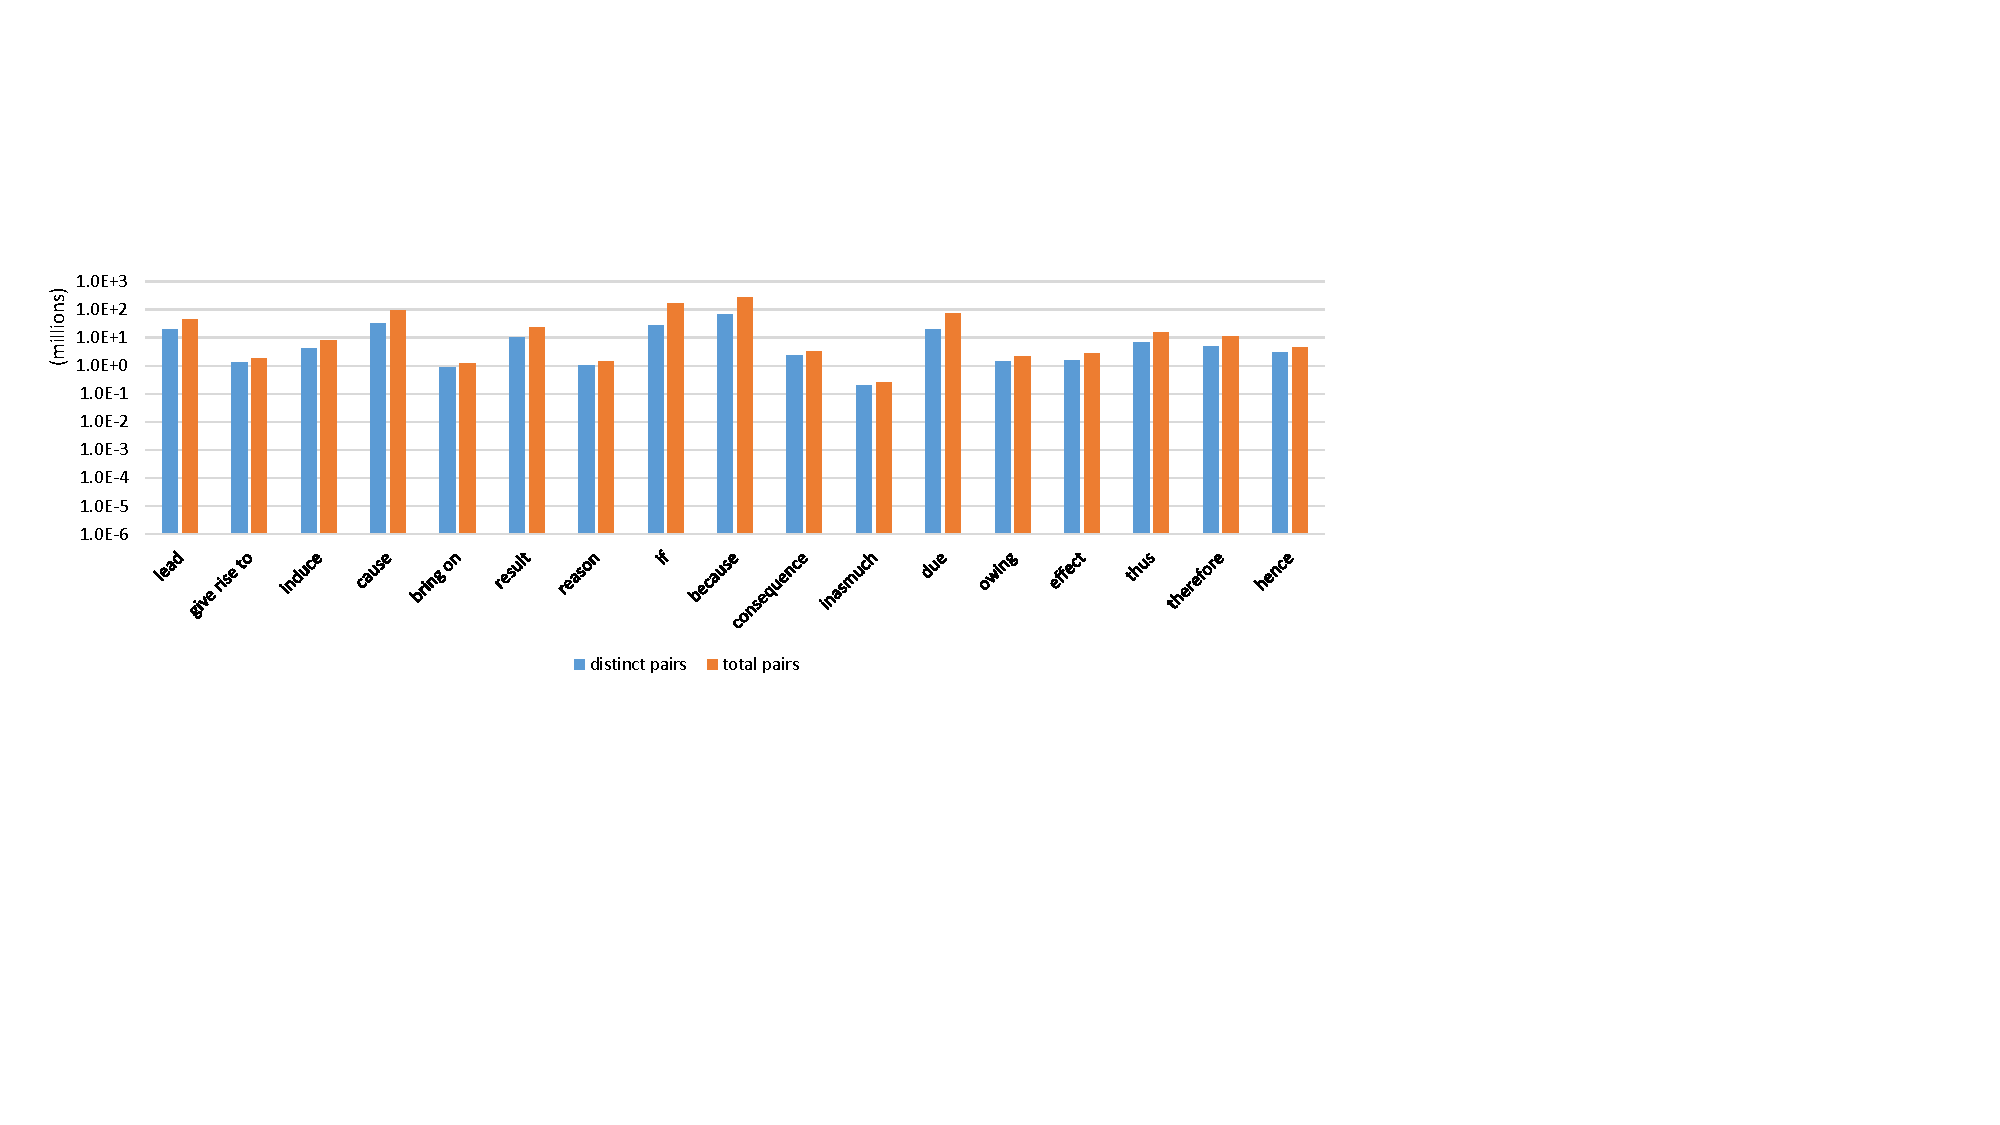
\includegraphics[width=2\columnwidth]{pattern.pdf}
% \caption{COPA Results by varying corpus size of Gutenberg }
%
% \label{fig:gu_pmi_1}
% \end{figure}

\subsection{Causality Detection}

Causality detection, or identifying the causal relation in text is 
an important task for many applications, such as event prediction, 
risk analysis, or decision making support\cite{mirza2014extracting}. 
To show the effectiveness of our work in this aspect, 
we investigate the following two research questions on 
CausalNet, using data from ConceptNet4.
\begin{itemize}
\item {\bf RQ1:}
For arbitrary event pair manually labeled as \emph{causal} (positive data)
or \emph{non-causal} (negative data), we investigate whether our
proposed causality strength score clearly separates the two.
\item {\bf RQ2:} Inspired by COPA, we select causal and non-causal pairs
sharing the same premise from ConceptNet and form two-choice
questions, to evaluate the ability of CausalNet in selecting the
correct choice.
\end{itemize}

%More specifically,
%we use \emph{pseudo-disambiguation task} used in~\cite{Erk}.
%Intuitively, ConceptNet, being manually generated, is limited in coverage,
%but expected to be near-perfect in precision.
%In particular, we follow Erk to use
%near-perfect causal event pairs $(u,v)$ from ConceptNet as positive ground-truth
%for testing, and to pair $u$
%with another random instance $v$ as negative ground-truth instances.

%The task is then to choose more likely effect $u$ among $v$ and $v'$
%using our network.
%(We can report precision and recall, and high score
%indicates that we are as good as ConceptNet in detection, with XX times larger
%coverage.
%Maybe we can show some pairs we found, as in your EMNLP draft if we are proud.)


For {\bf RQ1,}
%We do two applications based on ConcpetNet to show both reasonable of our
%causality metric on global causal pairs (thought it is difficult to give a
%threshold for causal relationship identification task) and usefulness to select
%plausible cause/effect from multiple-choice.
we use the same 200 causal and non-causal event pairs from
\figref{fig:pattern2} as positive and negative data.
%\ZY{For the ``Causes'' relation in
%ConcpetNet, people votes +1/-1 for event pairs in terms of particular relation
% to show their tendency whether the particular relation exists in the pair.
%The pairs with high positive votes (more than 3 in our experiment) in terms of
% ``Causes'' relation can be seen as positive examples, as those pairs with negative votes can be seen as negative examples.} Figure
\figref{fig:conceptApp1} shows the causality score ($y$-axis) of 100 positive
and negative pairs indexed randomly ($x$-axis). We can observe that scores
of positive and negative pairs are accurately distinguished by a
linear function, $y=10^{0}$, indicated by the gray line.
Consequently, existing systems for causality identification and detection 
can incorporate our work to improve their accuracy.

\begin{figure}[htb]
\centering
\epsfig{file=RQ1.eps, width=0.8\columnwidth}
\caption{Distinguishing causality on ConceptNet}
\label{fig:conceptApp1}
\end{figure}

For {\bf RQ2,} 
%we test our network in a COPA-like setting
%of classifying between causal and non-causal pairs sharing the
%same premise. 
due to sparsity of pairs sharing the same premise,
we follow \emph{pseudo-disambiguation task} in~\cite{Erk}.
%Intuitively, ConceptNet, being manually generated, is limited in coverage,
%but expected to be near-perfect in precision.
In particular, we use \emph{Causes} relationship $(i,j)$ with
positive votes, such that $i$ is the shared premise and $j$ is a
positive alternative. We then generate a negative alternative by
randomly selecting $j'$ without \emph{Causes} relationship with $i$.
%This approach is widely adopted in many tasks, as a large scale test
%cases can be generated, but as 
Since ConceptNet does not exhaustively
label all possible causal relationships, randomly selected $j'$ can
be actually causal, i.e., \emph{false negatives} may exist. In such
situation, we removed the question involving such false negative,
and consequently obtained a dataset of 412 questions in which 259
look for an effect while 153 look for a cause. \tabref{tab:rq2}
shows that the results of different $CS_\lambda$ 
using CausalNet.

\begin{table}[th]
%\small
\centering
\caption{Result of ConceptNet RQ2}
\begin{tabular}{cc}
%\hline CausalNet w/ events & CausalNet w/o events   \\ \hline \hline
\hline
Methods & Accuracy(\%) \\
\hline
$CS_{\lambda=0.5}$ & 78.4\%  \\
%$CS_{\lambda=0.7}$ & 79.6\%  \\
$CS_{\lambda=0.9}$ & 78.6\%  \\
$CS_{\lambda=1.0}$ & 78.6\%  \\
\hline
\end{tabular}
\label{tab:rq2}
\end{table}

%\ZY{We argue that to leverage explicit causality knowledge from web corpus, 
%empirical $\lambda$ set to be 0.7 with obtain rather good result on causality 
%reasoning for short texts, both phrases and sentences.}

\subsection{Direction of Causality}
%
%Causal relation is one form of relatedness. Thus,
%identifying a subset of causality from general relatedness is a
%challenge task. This section evaluates such ability of CausalNet via
%investigating its effectiveness of causality directional prior,
%since relatedness is a symmetric relation and causality is
%asymmetric.
%
Given a pair of terms $i$ and $j$ that are causally related,
CausalNet can generally tell whether the causality is encoded by $(i_c,j_e)$ 
or by $(j_c,i_e)$, without the context of
$i$ and $j$. In other words, as we will show next, CausalNet
provides a reasonable prior knowledge of causality direction.
We use the annotated corpus of SemEval-2010 Task 8 to evaluate this.
There are 920 pairs of terms annotated as Cause-Effect relationship in
SemEval-2010 Task 8 training corpus. CausalNet covered 894 out of
920 pairs (97.2\%). 
%Each Cause-Effect pair in the SemEval data set is annotated as follows:
%\begin{itemize}
%  \item[] Sentence:\\
%  {\em I too, get a $\langle e1\rangle$ \textbf{headache}$\langle/e1\rangle$ 
%  from $\langle e2\rangle$ \textbf{wine}$\langle/e2\rangle$, and was always told that it was the sulfites.}
%  \item[] Relation: \\ \emph{Cause-Effect($e2$,$e1$)}
%\end{itemize}
%In the above example, $e1$ represents the term ``headache'', and
%$e2$ represents ``wine''. The relation Cause-Effect($e2$,$e1$)
%indicates that the causality encoded in this sentence is
%\emph{wine}$ causes $ \emph{headache}, but not
%\emph{headache}$ causes $ \emph{wine}. We can obtain this useful
%insight by the prior knowledge from CausalNet.
We simply compare the causality strength of
$(i_c,j_e)$ with that of $(j_c,i_e)$ provided by
CausalNet. If $CS(i_c,j_e) > CS(j_c,i_e)$, we
conclude that the causality is encoded by $(i_c,j_e)$,
otherwise the causality is encoded by $(j_c,i_e)$. 

The agreement between CausalNet and annotated ground truth in SemEval-2010
Task 8 is 82.3\%, i.e., 736 out of 894 pairs from SemEval find 
a matching pair in the same causal direction from CausalNet.
Therefore, CausalNet provides high quality prior knowledge for
identifying causality direction 
%\tabref{tab:sample} shows 20 random samples of annotated causal pairs
%from SemEval-2010 Task 8 corpus. 10 of those are matched by
%CausalNet and the rest are not. Three human judges were employed to
%mark whether these pairs follow common sense or not. Those italicized pairs
%are considered common sense by at least 2 judges.
%We can see that all but one pairs in the left column are common sense,
%while most of those pairs in the right column are not common sense.
%This means, where CausalNet predicts correctly, it is really due to the power
%of commonsense knowledge. On the other hand, CausalNet makes mistakes primarily
%due to the lack of context in small amount of cases, and not because the
%knowledge enclosed is wrong.
\cut{
\begin{table}[th]
\centering
\caption{Random samples of annotated causal pairs from SemEval-2010 task 8}
\label{tab:sample}
\small
\begin{tabular}{|c c | c c |}
\hline \multicolumn{2}{|c|}{Pairs matched in CausalNet} &
\multicolumn{2}{c|}{Pairs not matched in CausalNet}\\
%\hline intra-sentence cue & inter-sentence cue  \\
\hline \hline
\multicolumn{1}{|c}{Cause} & \multicolumn{1}{c|}{Effect} & \multicolumn{1}{|c}{Cause} & \multicolumn{1}{c|}{Effect} \\
\hline
%\hline & \\
%\hline &\\
%A cause B & B caused by A & A induce B & If A, then B & A, hence B & A, thus B\\

\emph{vaccine} & \emph{fever}    & \emph{drink} & \emph{suffering} \\
\emph{tension} & \emph{headache}     & malfunction & inflammation\\
\emph{passage} & \emph{noise}    & growth & inflammation\\
\emph{injury} & \emph{discomfort}    & pie & poison\\
ash & drama  & city & anger\\
\emph{press} & \emph{reaction}   & \emph{infection} & \emph{acne}\\
\emph{extraction} & \emph{extinction}    & institution & fraud\\
\emph{mess} & \emph{crisis}  & dog & joy\\
\emph{pinworm} & \emph{infestation}  & fear & attack\\
\emph{parasite} & \emph{toxoplasmosis}   & \emph{bacteria} & \emph{acne}\\
\emph{disability} & \emph{benefit}   & \emph{fireplace} & \emph{warmth}\\
%\emph{elimination} & \emph{riot}     & tax & fluctuation\\
%\emph{generator} & \emph{signal}     & \emph{bacteria} & \emph{breakout}\\
%\emph{drug} & \emph{unconsciousness}     & \emph{injury} & \emph{operation}\\
%\emph{zinc} & \emph{growth}  & \emph{pregnancy} & \emph{nausea}\\
%\emph{reaction} & \emph{inversion}   & \emph{attack} & \emph{shock}\\
%\emph{movement} & \emph{earthquake}  & lack & reliance\\
%\emph{virus} & \emph{disease}    & computer & radiation\\
%\emph{drum} & \emph{sound}   & ointment & discomfort\\
%\emph{vaccine} & \emph{outbreak}     & ginseng & taste\\
\hline
\end{tabular}
\end{table}
}
%CausalNet provides pretty (pretty?) good prior knowledge for commonsense
%causality, since we do not use other local context information.
%This shows that CausalNet can effectively tell the difference
%from relatedness and causality.

%\begin{figure*}[th]
%\centering
%\begin{subfigure}[t]{0.9\columnwidth}%0.7\columnwidth
%\centering
%\epsfig{file=f1.eps, width=0.9\columnwidth, angle=0,
%clip}%width=0.4\columnwidth, angle=270
%\caption{flood}
%\end{subfigure}
%\begin{subfigure}[t]{0.9\columnwidth}
%\centering
%\epsfig{file=f2.eps, width=0.9\columnwidth, angle=0, clip}
%\caption{cancer}
%\end{subfigure}
%\begin{subfigure}[t]{0.9\columnwidth}
%\centering
%\epsfig{file=f3.eps, width=0.9\columnwidth, angle=0, clip}
%\caption{debt}
%\end{subfigure}
%\begin{subfigure}[t]{0.9\columnwidth}
%\centering
%\epsfig{file=f4.eps, width=0.9\columnwidth, angle=0, clip}
%\caption{angry}
%\end{subfigure}
%\begin{subfigure}[t]{0.9\columnwidth}
%\centering
%\epsfig{file=f5.eps, width=0.9\columnwidth, angle=0, clip}
%\caption{headache}
%\end{subfigure}
%\begin{subfigure}[t]{0.9\columnwidth}
%\centering
%\epsfig{file=f6.eps, width=0.9\columnwidth, angle=0, clip}
%\caption{guilty}
%\end{subfigure}
%%
%%\subfigure[]{\epsfig{file=ex2.eps, width=0.25\columnwidth, angle=270, clip}}
%%\subfigure[]{\epsfig{file=ex3.eps, width=0.25\columnwidth, angle=270, clip}}
%%\subfigure[]{\epsfig{file=ex4.eps, width=0.25\columnwidth, angle=270, clip}}
%%\subfigure[]{\epsfig{file=ex5.eps, width=0.25\columnwidth, angle=270, clip}}
%%\subfigure[]{\epsfig{file=ex6.eps, width=0.25\columnwidth, angle=270, clip}}
%%\subfigure[]{\scalebox{0.42}{\includegraphics[angle=270,clip]{ex1.eps}}}
%%\subfigure[]{\scalebox{0.42}{\includegraphics[angle=270,clip]{ex2.eps}}}
%%\subfigure[]{\scalebox{0.42}{\includegraphics[angle=270,clip]{ex3.eps}}}
%%\subfigure[]{\scalebox{0.42}{\includegraphics[angle=270,clip]{ex4.eps}}}
%%\subfigure[]{\scalebox{0.42}{\includegraphics[angle=270,clip]{ex5.eps}}}
%%\subfigure[]{\scalebox{0.42}{\includegraphics[angle=270,clip]{ex6.eps}}}
%\caption{Examples from CausalNet demo}
%\label{fig:example1}
%\end{figure*}



%More examples of ConceptNet (and a complete ranking of causal words)  can be
%found from \url{http://202.120.38.146/causal/causalnet.html} ,

%\subsection{Discussion}
%\label{sec:discuss}
%\begin{figure}[th]
%\centering
%\epsfig{file=snapshot.eps,width=\columnwidth}
%\caption{A snapshot of the demo}
%\label{fig:snapshot}
%\end{figure}
%
%The complete demo includes 2881 unique lemmatized words that ever appear
%in the COPA data set. Stanford NLP tools \cite{chen2014fast} were used for
%lemmatization. Topics in COPA data set were drawn from
%different sources\cite{roemmele2011choice} to ensure comprehensive coverage
%of different domains.
% want to show some results and talk about existing issues in our work
%To further illustrate CausalNet, we give some concrete
%examples from our demo (with a snapshot shown in \figref{fig:snapshot}).
%Arrows shown in
%\figref{fig:example1} indicate the directions of causality.
%\figref{fig:example1} (a),(b),(c),(d),(e) and (f) show the top 5 ranked
%causes and effects of the terms, ``flood'', ``cancer'', ``debt'',
%``angry'', ``headache'', and ``guilty'', respectively.
%
%Capturing commonsense causal relations for all words is
%an ambitious goal.
%While CausalNet generally gives reasonable causes and effects
%for most common words,
%there are still noises and errors.
%%Our end-to-end COPA evaluation accuracy is still below 70\%.
%For example, in \figref{fig:example1} (d), ``wet'' and ``hug'' rank ahead of
%``insult'' as the causes of ``angry'', which is counter-intuitive to most
%people.
%This section we show analysis our extracted commonsense causal knowledge.
% Although, we introduced techniques to solve
%It's really a challenging task to get pretty robust causality ranking
%results. As \figref{fig:example1} (d) shown, the term ``wet'' ranks higher than
%``insult''.
%CausalNet is inevitably biased toward terms with high popularity in
%common sense. Relative reasonable results are acceptable
%for commonsense causal reasoning.

\cut{%%%%%%%%%%%%%%%
Our preliminary analysis shows that these noises and errors are due to
two limitations of our approach.

First, CausalNet is constructed on individual words only, but many events
cannot be effectively encoded in a single word. For example, our investigation
shows that \emph{hug} $\rightarrow$ \emph{angry} in \figref{fig:example1} (d)
is likely extracted from patterns such as
``because...refuse to hug, ... angry''. In fact, our extracted pair
 \emph{hug} $\rightarrow$ \emph{angry} is only part of a ``negative''
causal relation $not~ hug \rightarrow angry$. Fortunately, while some
of the causal word pairs from CausalNet do not appear very rational in their
own right, when used with other pairs together,
the combined causal strength can provide
reasonable commonsense reasoning between more complex text units.

Second, pattern-based extraction has its limitation.
The 53 causal cues we used to extract CausalNet are indicative of
a potential causal relation in the text. But this is not always true.
For example, ``$A$ rarely causes $B$'' matches one of the cues but is certainly
not causality. This kind of situation gives rise to many false positives in
CausalNet. Furthermore, causal cues do not capture implicit causality.
People may say ``I'm not hungry, I just had lunch.'' instead of
``I'm not hungry because I just had lunch.'' Such implicit causal knowledge
is currently ignored by our approach.
Existing approaches, such as \cite{ittoo2011extracting}, attempted to
obtain implicit causality on domain-specific texts.
But such work can not easily extend to open
domain causality acquisition due to the introduction of excessive noise.
%More efforts need to be done on this part.
Our work essentially strikes a trade-off between simplicity and
refinement. Even though the causal cues are not refined enough to
identify all the causality knowledge there is in the corpus, the
simplicity of the approach enables us to work on data of much larger
scale, which to some extent makes up for the deficiency of the
framework.

}%%%%%%%%%%%%%% end of cut %%%%%%%%%%%%

% 
%This is a trade-off consideration. Although the
%causal cues cannot detect some of the implicit causal relations in text,
%the large scale of the input data somewhat \ZY{more or less?} makes up for this
%deficiency.
%We will make effort to develop effective approach which can
%properly leverage implicit causal knowledge for commonsense causal reasoning
%task in future.

%
%Another issue exists in CausalNet is that we can not
%identify the correct polarity from extracted causal pairs. The reason is that we
%ignored false causality and anti-causality during causal relation extraction.
%We extract false causality ``A $\rightarrow$ B'' from sentence like `` A
%rarely causes B''.
%%For example, \emph{treat} $\rightarrow$
%%\emph{disease} has a very high causal strength in CausalNet, but the real
%%causality encoded in text is more likely to be \emph{treat} $\rightarrow$
%%\emph{eliminate disease}.
%For anti-causality, as shown in \figref{fig:example1} (d), the term \emph{hug}
%causes/implies \emph{angry} which is a little strange. But if we have the ability to
%identify it as anti-causality, but the real
%causality encoded in text is more likely to be \emph{refuse
%to hug} $\rightarrow$ \emph{angry} other than \emph{hug} $\rightarrow$ \emph{anger}.
%We do not distinguish these false causality and anti-causality in CausalNet.
%Thus, CausalNet can not tell the polarity of causality.
%Identifying anti-causality which involves much more complex knowledge is a
%harder task and incorporating these is a possible future work.
%
%For example, Our framework calculated
%idf weight to penalize terms with high popularity and will somewhat make up for
% this deficiency.
%There are two major issues which need further consideration.
